%%
%  ******************************************************************************
%  * #file    Szablon_raportu_EN_Latex.tex
%  * #author  Adrian Wójcik   adrian.wojcik(at)put.poznan.pl
%  *          
%  * #commit  Patryk Kościk   koscikpatryk(at)gmail.com
%  *          Modified the template for Projekt przejsciowy purposes          
%  *          
%  * #version 1.0
%  * #date    09-Mar-2022
%  * #brief   PROJPRZEJ
%  *
%  ******************************************************************************
%%  
\documentclass[11pt, a4paper]{article}

\usepackage{SM_template}

% Wypełnijcie te dyrektywy zgodnie z waszym tematem
% \lab      -> NAZWA CZUJNIKA, np.: 'DHT22'
% \comment  -> Króciutki opis co to, np.: 'Cyfrowy budżetowy czujnik temperatury'
%

\lab{DA5883}
\comment{3-osiowy cyfrowy kompas magnetometr}
\author{Antoni Borowski}
\addbibresource{bib/DA5883.bib}

% Absolutny zakaz dotykania tego tutaj bo jak dotkiecie to coś jebnie
\university{Politechnika Poznańska}
\faculty{Wydział Automatyki, Robotyki i Elektrotechniki}
\institute{Instytut Robotyki i Inteligencji Maszynowej}
\department{Zakład Sterowania i Elektroniki Przemysłowej}

\nocite{*}


%%
%
% Początek dokumentu
%
%%
\begin{document}

%% Strona tytułowa %%
\mainpage{{DA5883/foto}}
\newpage

\section*{Opis elementu} \addcontentsline{toc}{section}{Wstęp}
QMC5883L jest cyfrowym, 3-osiowym magnetometrem. Odczyt danych wykonywany jest poprzez magistralę I$^{2}$C. Przeznaczony jest do pomiaru szerokiego zakresu wielkości pola magnetycznego Ziemi. Układ ten pozwala na osiągnięcie częstotliwości pomiarów siegającej nawet 160Hz w trybie pojedynczego pomiaru. Posiada możliwość wyboru ilości próbek, które podlegają uśrednieniu końcowego wyniku.
Mimo, że na PCB nadrukowane jest HMC5883L istnieją dwa warianty opisywanego układu - jeden wykorzystuje HMC5883L, a drugi QMC5883L. Różnią się one kilkoma istotnymi względami. Przed użyciem należy sprawdzić którą wersje posiadamy. Można to zrobić poprzez odczytanie numeru nadrukowanego na centralnym układzie scalonym (L883 oznacza HMC5883L, a 5883 ozancza QMC5883L).
W tym dokumencie opisany zostanie QMC5883L.\\
\vspace{0.5cm}
\begin{figure}[h!]
    \centering
    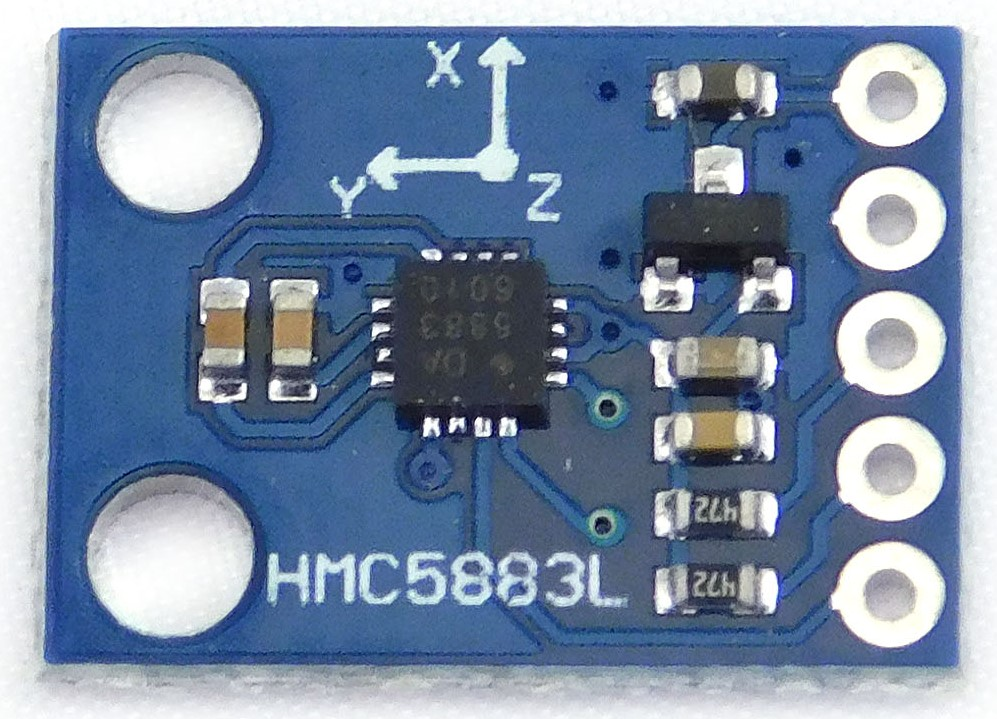
\includegraphics[width=0.4\textwidth]{fig/DA5883/zdj_modułu/modul.jpg}
    \caption{Moduł z innym układem niż podpisano \cite{ArduinoModules:grab}}
    \label{fig:my_label}
\end{figure}
\newline
Sam moduł składa się z magnetometru (HMC5883L lub QMC5883L), dwóch rezystorów, pięciu kondensatorów, regulatora napięcia oraz pięciu wyprowadzeń w postaci pinów męskich.
\vspace{0.5cm}
\begin{figure}[h!]
    \centering
    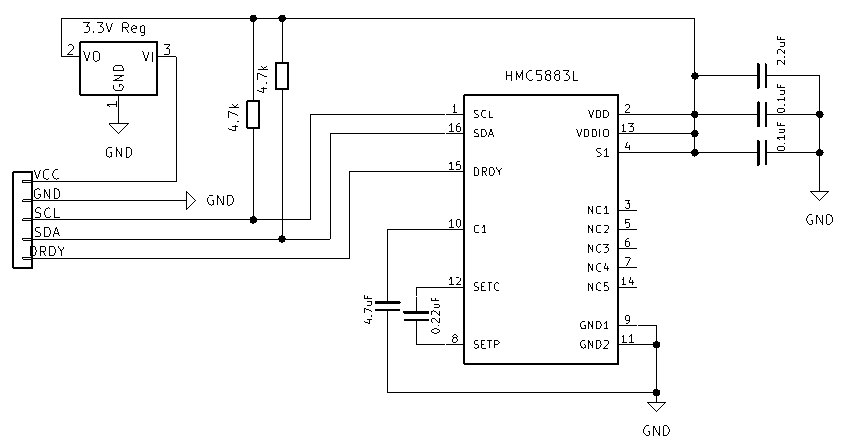
\includegraphics[width=.95\textwidth]{fig/DA5883/polaczenie_modulu/schemat.png}
    \caption{Schemat modułu}
    \label{fig:my_label}
\end{figure}
\newpage
\section*{Użycie czujnika}
W celu użycia czujnika należy skorzystać z interfejsu I$^{2}$C. Podstawowym adresem tego czujnika jest 0x0D. Czujnik posiada 14 rejestrów.
\begin{table}[h!]
\centering
\begin{tabular}{|c|cccccccc|c|}
\hline
Adres &
  \multicolumn{1}{c|}{7} &
  \multicolumn{1}{c|}{6} &
  \multicolumn{1}{c|}{5} &
  \multicolumn{1}{c|}{4} &
  \multicolumn{1}{c|}{3} &
  \multicolumn{1}{c|}{2} &
  \multicolumn{1}{c|}{1} &
  0 &
  Dostęp \\ \hline
00H &
  \multicolumn{8}{c|}{Oś X LSB[7:0]} &
  Odczyt \\ \hline
01H &
  \multicolumn{8}{c|}{Oś X MSB[15:8]} &
  Odczyt \\ \hline
02H &
  \multicolumn{8}{c|}{Oś Y LSB[7:0]} &
  Odczyt \\ \hline
03H &
  \multicolumn{8}{c|}{Oś Y MSB[15:8]} &
  Odczyt \\ \hline
04H &
  \multicolumn{8}{c|}{Oś Z LSB[7:0]} &
  Odczyt \\ \hline
05H &
  \multicolumn{8}{c|}{Oś Z MSB[15:8]} &
  Odczyt \\ \hline
06H &
  \multicolumn{1}{c|}{} &
  \multicolumn{1}{c|}{} &
  \multicolumn{1}{c|}{} &
  \multicolumn{1}{c|}{} &
  \multicolumn{1}{c|}{} &
  \multicolumn{1}{c|}{DOR} &
  \multicolumn{1}{c|}{OVL} &
  DRDY &
  Odczyt \\ \hline
07H &
  \multicolumn{8}{c|}{Temperatura LSB[7:0]} &
  Odczyt \\ \hline
08H &
  \multicolumn{8}{c|}{Temperatura MSB[15:8]} &
  Odczyt \\ \hline
09H &
  \multicolumn{2}{c|}{OSR[1:0]} &
  \multicolumn{2}{c|}{RNG[1:0]} &
  \multicolumn{2}{c|}{ODR[1:0]} &
  \multicolumn{2}{c|}{MODE[1:0]} &
  Odczyt/Zapis \\ \hline
0AH &
  \multicolumn{1}{c|}{SOFT\_RST} &
  \multicolumn{1}{c|}{ROL\_PNT} &
  \multicolumn{1}{c|}{} &
  \multicolumn{1}{c|}{} &
  \multicolumn{1}{c|}{} &
  \multicolumn{1}{c|}{} &
  \multicolumn{1}{c|}{} &
  INT\_ENB &
  Odczyt/Zapis \\ \hline
0BH &
  \multicolumn{8}{c|}{SET/RESET Period FBR [7:0]} &
  Odczyt/Zapis \\ \hline
0CH &
  \multicolumn{8}{c|}{Reserved} &
  Odczyt \\ \hline
0DH &
  \multicolumn{8}{c|}{Reserved} &
  Odczyt \\ \hline
\end{tabular}
\caption{Tabela rejestrów}
\end{table}

\begin{itemize}
\item Pierwsze 6 (00H-05H) służy do odczytu danych z poszcególnych osi magnetometru. Dane mają postać liczby 16-bitowej podzielonej na dwa rejestry 8-bitowe.
\item Rejestr 06H jest rejestrem statusowym przechowującym trzy flagi,
\item Rejestry 07H oraz 08H przechowują aktualny odczyt temperatury, który jest liczbą 16-bitową podzieloną na dwa rejestry-8 bitowe.
\item Rejestry 09H oraz 0AH są dwoma rejestrami kontrolnymi, które służą do sterowania czujnikiem.
\begin{itemize}
    \item Mode definiuje tryb pracy czujnika - 00 oznacza, że czujnik jest w stanie Standby a 01, że wykonuje ciągłe pomiary.
    \item ODR definuje jak często wykonywane są pomiary (00-10Hz, 01-50Hz, 10-100Hz, 11-200Hz).\\
    \item RNG definiuje zakres pomiaru magnetometru (00-2G 01-8G).\\
    \item OSR oznacza Over Sample Ratio (00-512, 01-256, 10-128, 11-64).\\
    \item Kiedy INT\_ENB jest ustawione na 1, to wtedy, gdy bedą gotowe nowe dane do odczytu, pojawi się stosowna flaga.\\
    \item Ustawienie flagi ROL\_PNT skutkuje tym, że w przypadku rozpoczęcia odczytu danych z innego rejestru niż 00H, będzie skutkowało zawinięciem na początek rejestrów z danymi.\\
    \item SOFT\_RST służy do ustawienia podstawowych wartości rejestrów.\\
\end{itemize}
\item Rejestr 0BH służy do ustawienia SET/RESET period.
\item Rejestry 0CH i 0DH są zarezerwowane dla wewnętrznych operacji czujnika.
\end{itemize}
\vspace{0.5cm}

Przed przystąpieniem do pracy należy zapisać odpowiednie wartości do rejstrów kontrolnych tak, aby odpowiadały naszym potrzebom. Następnie należy dokonywać cyklicznego odczytu flagi DRDY i kiedy ta jest ustawiona na 1, dokonywać odczytu rejestrów z danymi. Warto zwrócić uwagę na to, że aby uzyskać poprawny pomiar orientacji w płaszczyźnie XY, należy dodać przesunięcie pomiarów z czujnika w taki sposób, by charakterystyka z pełnego obrotu była wyśrodkowana względem punktu 0.0, a następnie skorzystać z funkcji $atan$. Konieczność dodania przesunięcia wynika z obecności zakłóceń elektromagnetycznych. Z tego powodu to przesunięcie nie jest stałe i zależy od środowiska. Dodatkowo, jeśli występują duże ilości fal elektromagnetycznych, pomiary mogą być znacznie zaszumione. Oprócz tego, ferromagnetyki w srodowisku mimo, że same nie wytwarzają pola, to zakrzywiają pole ziemskie, co może skutkować niepoprawnym wskazaniem bieguna.
\vspace{0.5cm}
\begin{figure}[h!]
    \centering
    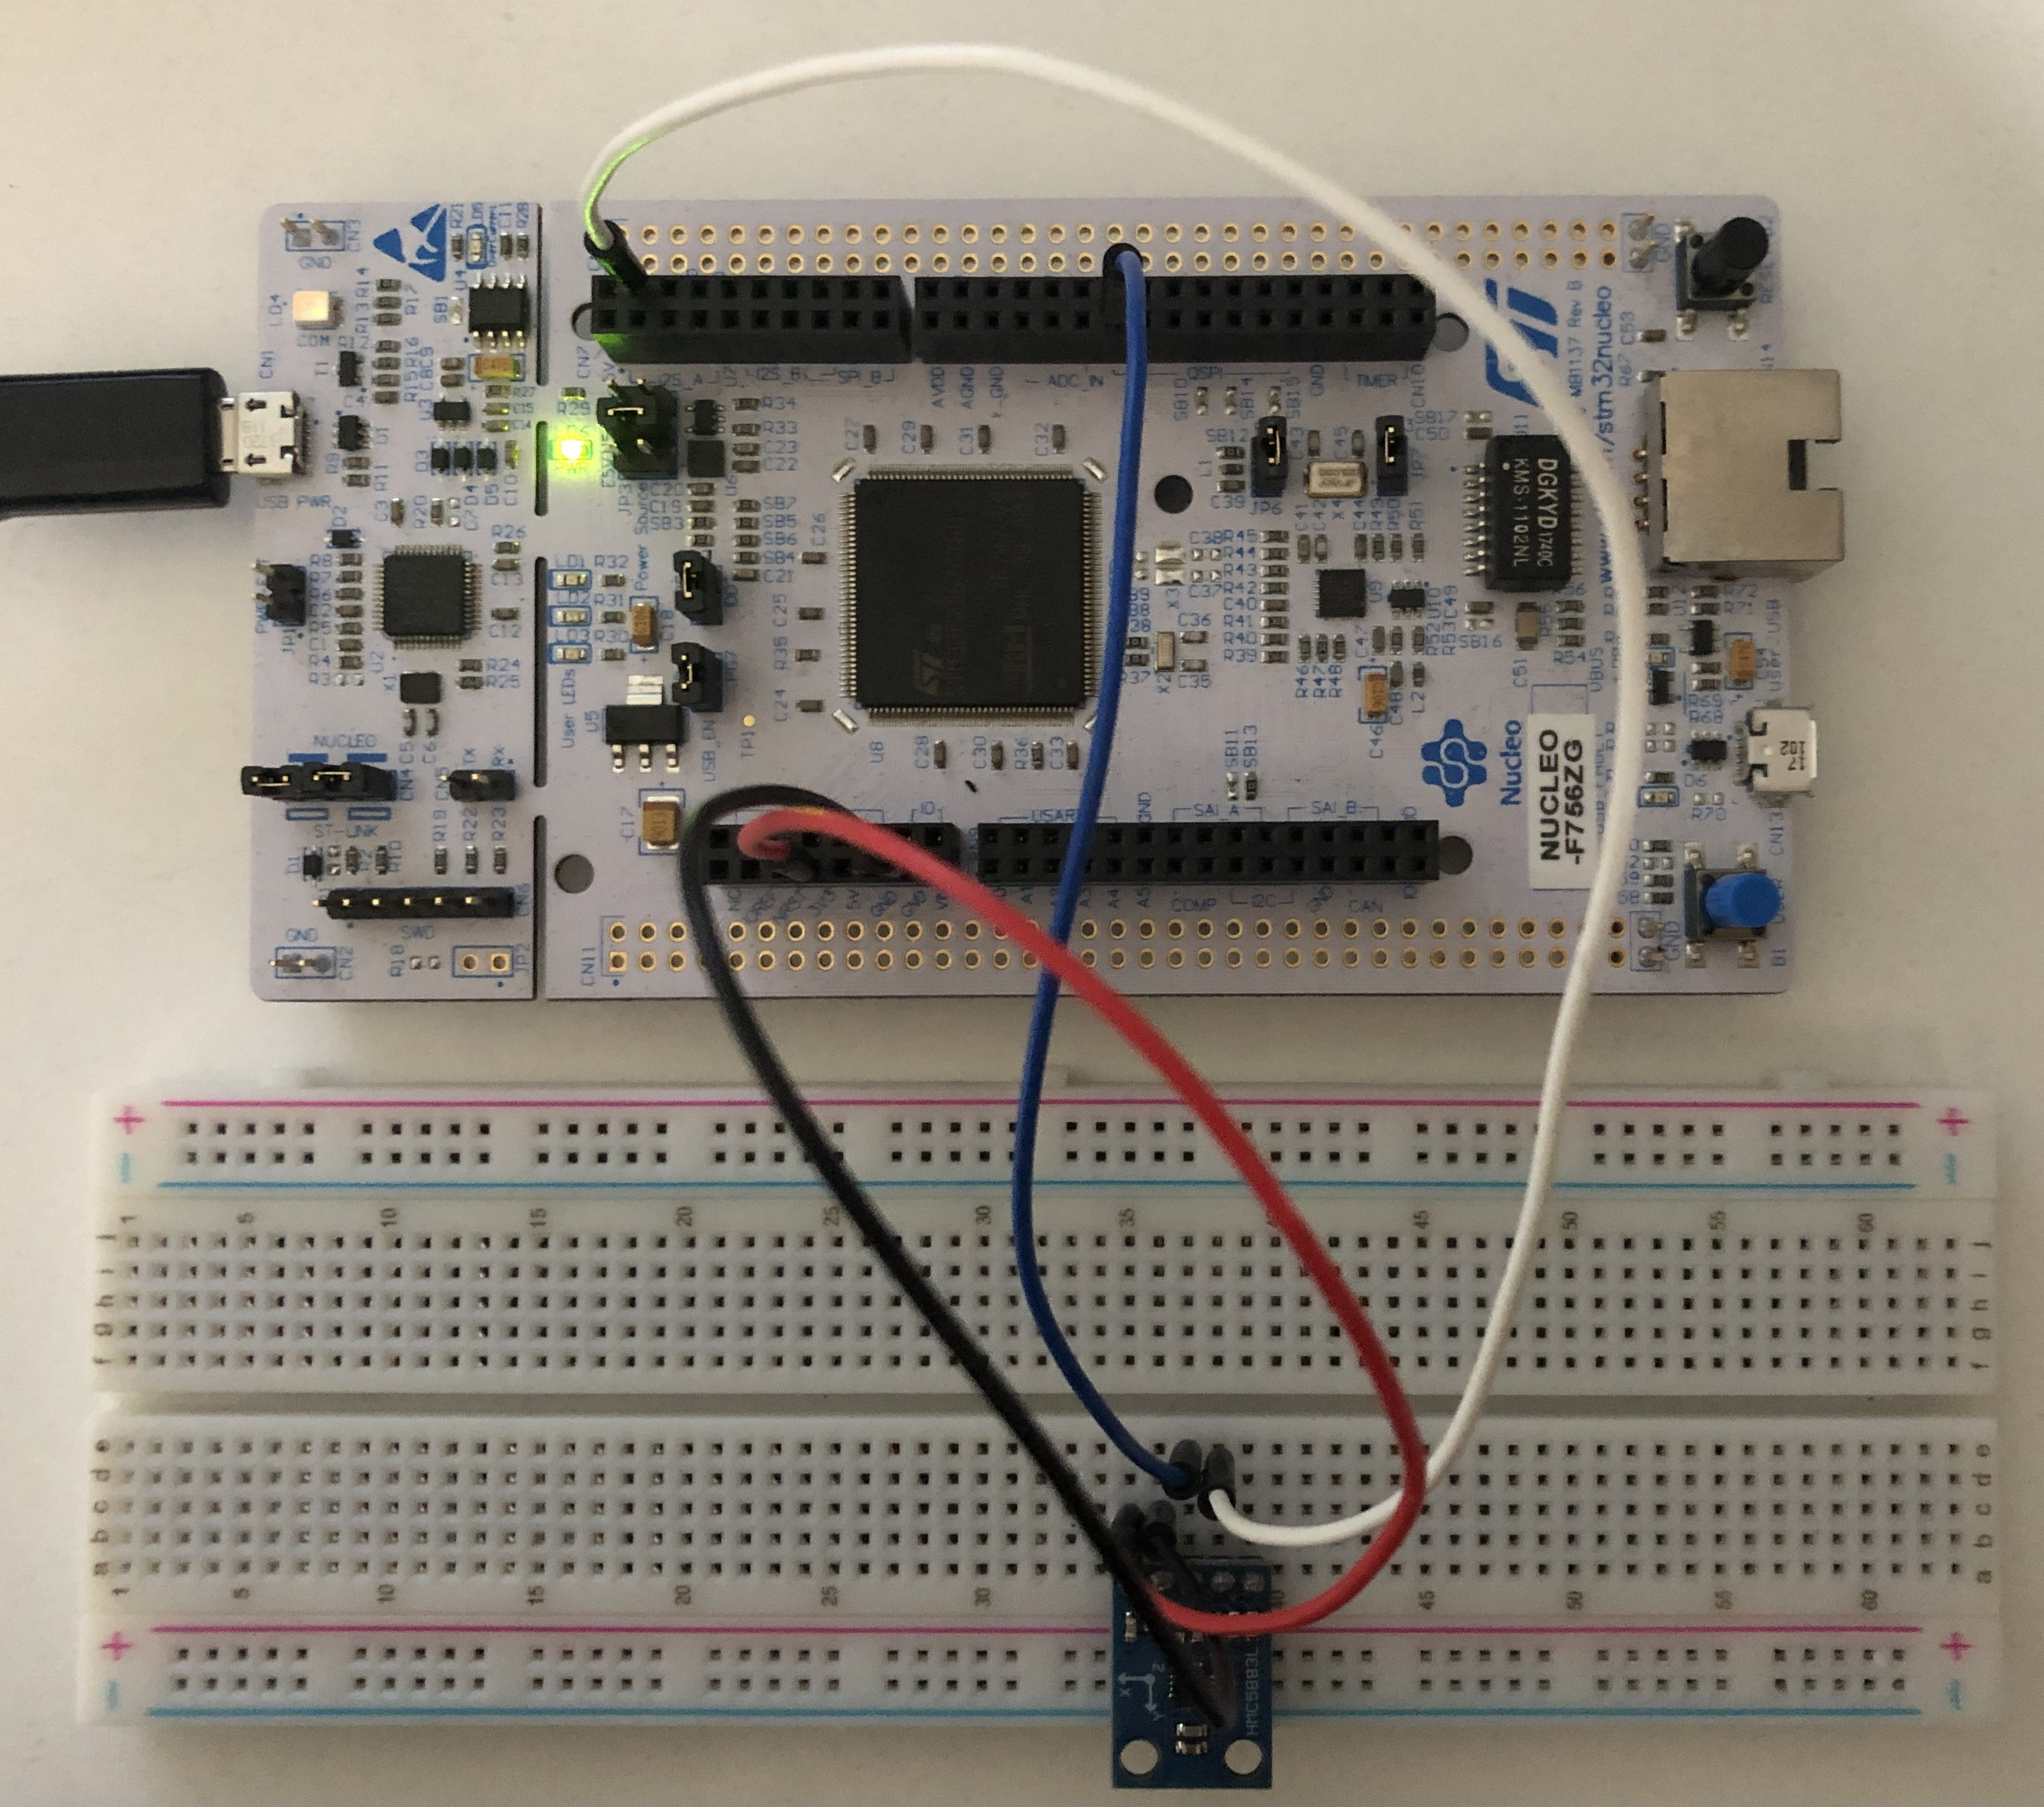
\includegraphics[width=.6\textwidth]{fig/DA5883/polaczenie_modulu/uklad.jpg}
    \caption{Podłączenie modułu}
    \label{fig:my_label}
\end{figure}
\newline
Po poprawnym oprogramowaniu czujnika, możemy odczytywać wartości położenia różnych osi.
\begin{figure}[h!]
\centering
\begin{subfigure}{.5\textwidth}
  \centering
  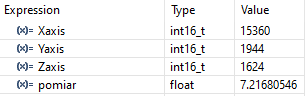
\includegraphics[width=1\linewidth]{fig/DA5883/działanie_ukladu/wartosci.png}
  \caption{Pomiar równolegle do podłoża}
  \label{fig:sub1}
\end{subfigure}%
\begin{subfigure}{.5\textwidth}
  \centering
  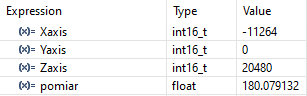
\includegraphics[width=1\linewidth]{fig/DA5883/działanie_ukladu/wartosci2.png}
  \caption{Pomiar prostopadle do podłoża}
  \label{fig:sub2}
\end{subfigure}
\caption{Odczyty czujnika w zależności od jego położenia}
\label{fig:test}
\end{figure}
\newline
Kod programujący czujnik, wykorzystany do opracowania instrukcji, znajduje się w materiałach dodatkowych zawartych pod koniec rozdziału.
\newline

Film prezentujący działanie układu znajduje się w suplemencie wideo.
\printbibliography[heading=bibintoc]

\end{document}